\section{Dijkstras Algoritme}

Dijkstras algoritme er en algoritme til at finde den korteste vej fra et bestemt punkt til et andet punkt. Disse punkter kan bland andet repræsentere den korteste vej mellem to forskellige byer. Dijkstra fungerer på nogenlunde samme måde som A* i dens planlæggende fremgangsmåde ved at sammenligne punkter med hinanden. Dijkstras algoritme skanner også et område af kasser fra et startpunkt og fortsætter som eksemplificeret i figur \ref{fig:AKvadrat2}. Dijkstra modtager dog ikke heuristiske datasæt Dijkstras er en grådig algoritme, da den finder den korteste længde først og fortsætter således.\cite{DMATBOGEN} Dette kaldes også Greedy Best First Search.

\vspace{5mm}

Dijkstras algoritme finder den korteste rute mellem 2 forskellige punkter i en simpel ikke-orienteret vægtet graf. Man kan se på figur \ref{fig:dijkstrasgraf} at der angives forskellige punkter {A, B, C, D, E, Z}. Hvis man skal fra punkt A til Z på figuren, så starter man ved A og derfor initialiseres A til at være 0, som man kan se på tabel \ref{fig:dijkstratabel}. Algoritmen virker således, at alle punkter er uendeligt udover det punkt man befinder sig på som vist på tabel \ref{fig:dijkstratabel}. Algoritmen tager punkt fra punkt, så den starter med at se de grene som A har. Disse er |AB| = 4 og |AC| = 2. Her fra kan algoritmen ikke se videre end B og C. Den ser altid på det mindste tal, og derfor tager den længden fra A til B som er 4 og længden fra A til C som er 2, begge disse tal er mindre end uendeligt. Herefter ser den efter hvilket af de nuværende tal som er mindst, hvilket er 2. Så derfor vælger den C som sit næste punkt. Algoritmen finder nu de næst tætteste punkt, ved at addere alle de tidligere ruter, som har den korteste rute fra A til det næste sæt af punkter. Her ser algoritmen ud fra C og hvilke grene C har. Dette er længden til B, D og E, dog er længden altid fra A, så derfor er længden fra A til E 12 da 2+10 = 12. Længden til B er nu blivet 3, da algoritmen ser på den korteste rute, så A til B er 3, da 2+1 = 3. Således fortsætter algoritmen indtil den rammer Z.\cite{DMATBOGEN}

\begin{figure}[H]
\begin{adjustbox}{width=1.2\textwidth,center=\textwidth}
\centering
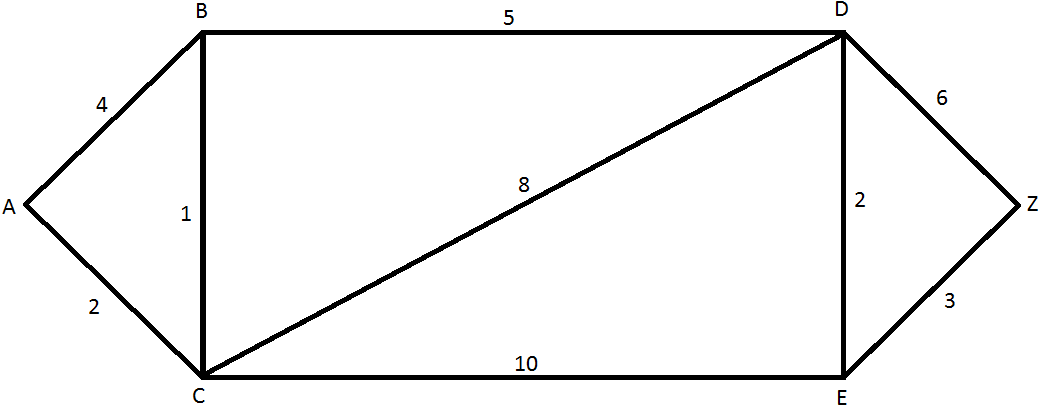
\includegraphics[width=1.2\textwidth]{Pictures/Teoriafsnit/Figurfiler/dijkstrasgraf.png}
\end{adjustbox}
\caption{Graf til fremvisning af eksempel af Dijkstras algoritme i brug}
\label{fig:dijkstrasgraf}
\end{figure}

\begin{table}[H]
\centering
\begin{adjustbox}{width=1\textwidth}
\Large
\begin{tabular}{| c | c | c | c | c | c | c |}
	\hline
	 & A & B & C & D & E & Z \\
	\hline
	 & 0 & Inf & Inf & Inf & Inf & Inf \\
	\hline
	{A} & 0 & 4 & 2 & Inf & Inf & Inf \\
	\hline
	{A, C} & 0 & 3 & 2 & 10 & 12 & Inf \\
	\hline
	{A, C, B} & 0 & 3 & 2 & 8 & 12 & Inf \\
	\hline
	{A, C, B, D} & 0 & 3 & 2 & 8 & 10 & 14 \\
	\hline
	{A, C, B, D, E} & 0 & 3 & 2 & 8 & 10 & 13 \\
	\hline
	{A, C, B, D, E, Z} & 0 & 3 & 2 & 8 & 10 & 13 \\
	\hline
\end{tabular}
\end{adjustbox}
\caption{Dijkstra tabel}\label{fig:dijkstratabel}
\end{table}

\begin{lstlisting}[language=C,caption={Dijkstras angivet som eksempel i pseudo-kode},label={lst:DijsktrasPseudo1}]
	procedure Dijkstras(G: weighted connected simple graph, with all weights positive)
{G has vertices a = V0, V1, ....... Vn = z and lengths w(Vi, Vj) where w(Vi,Vj) = infinity if{Vi, Vj} is not an edge in G}
for (i = 1 to n)
	L(Vi) = infinity
L(a) = 0
S = NULL
{ the labels are now initialized so that the label of a is 0 and all other labels are infinity, and S is the empty set }
while (z does not belong to S)
	u = a vertex not in S with L(u) minimal
	S = S U {u}
	for (all vertices v not in S)
		if (L(u) + w(u, v) < L(v) then L(v) = L(u) + L(u, v))
		{this adds a vertex to S with minimal label and updates the labels of vertices not in S}
return (L(z)) {L(z) = length of a shortest path from 	a to z}
\end{lstlisting}